\documentclass{article}
\usepackage{graphicx} % Required for inserting images
\usepackage{polyglossia} % used to display different languages
\usepackage{enumitem}
\usepackage{nameref}
\usepackage{fontspec}
\usepackage[dvipsnames]{xcolor}

\setdefaultlanguage{greek}
\setotherlanguage{english}
\newfontfamily\greekfont{Arial}


\usepackage{fancyhdr} % used for custom headers

\pagestyle{fancy} % allow the creation of custom headers
\fancyhf{} % clear existing footers and headers
\setlength{\headheight}{1cm}
\rhead{
    Airline Manager Template
    
\includegraphics[height=0.8cm, keepaspectratio]{image.png}
}

\title{
    
\includegraphics[height=1cm, keepaspectratio]{image.png}
    SkyOps - use cases v0.3
}
\author{}

\date{} % date displayed underneath title

\setlength{\parskip}{16pt}


% document specific commands
\newcounter{counterBasicFlow}
\newcounter{counterAlternativeFlow}[counterBasicFlow]
\newcommand{\bFlowIDReset}{\setcounter{counterBasicFlow}{0}}
\newcommand{\bFlowID}{\protect\stepcounter{counterBasicFlow}\thecounterBasicFlow}
\newcommand{\basicFlow}{\subsection*{Βασική Ροή \bFlowID}}
\newcommand{\basicFlowNew}{\bFlowIDReset\basicFlow}
\newcommand{\alternativeFlow}[1][]{\subsection*{Εναλλακτική #1 Ροή \protect\stepcounter{counterAlternativeFlow}\thecounterAlternativeFlow}}
\newcommand{\flowbody}[2]{
\begin{enumerate}[label=#1\arabic*]
#2
\end{enumerate}
}
\newcommand{\docChange}[1]{\textcolor{red}{#1}}



\begin{document}

\maketitle

\newpage
Χρήστος Καπετανάκης 1103828 \\
Ανδρέας Κρητικός 1104781 \\
Γιώργος Τεμπονέρας 1104775 \\
Ελευθερία Γιαννοπούλου 1041039 \\
Αλέξης Λούμπαρδης 1051948
\newpage

\begin{figure}[h]
    \centering
    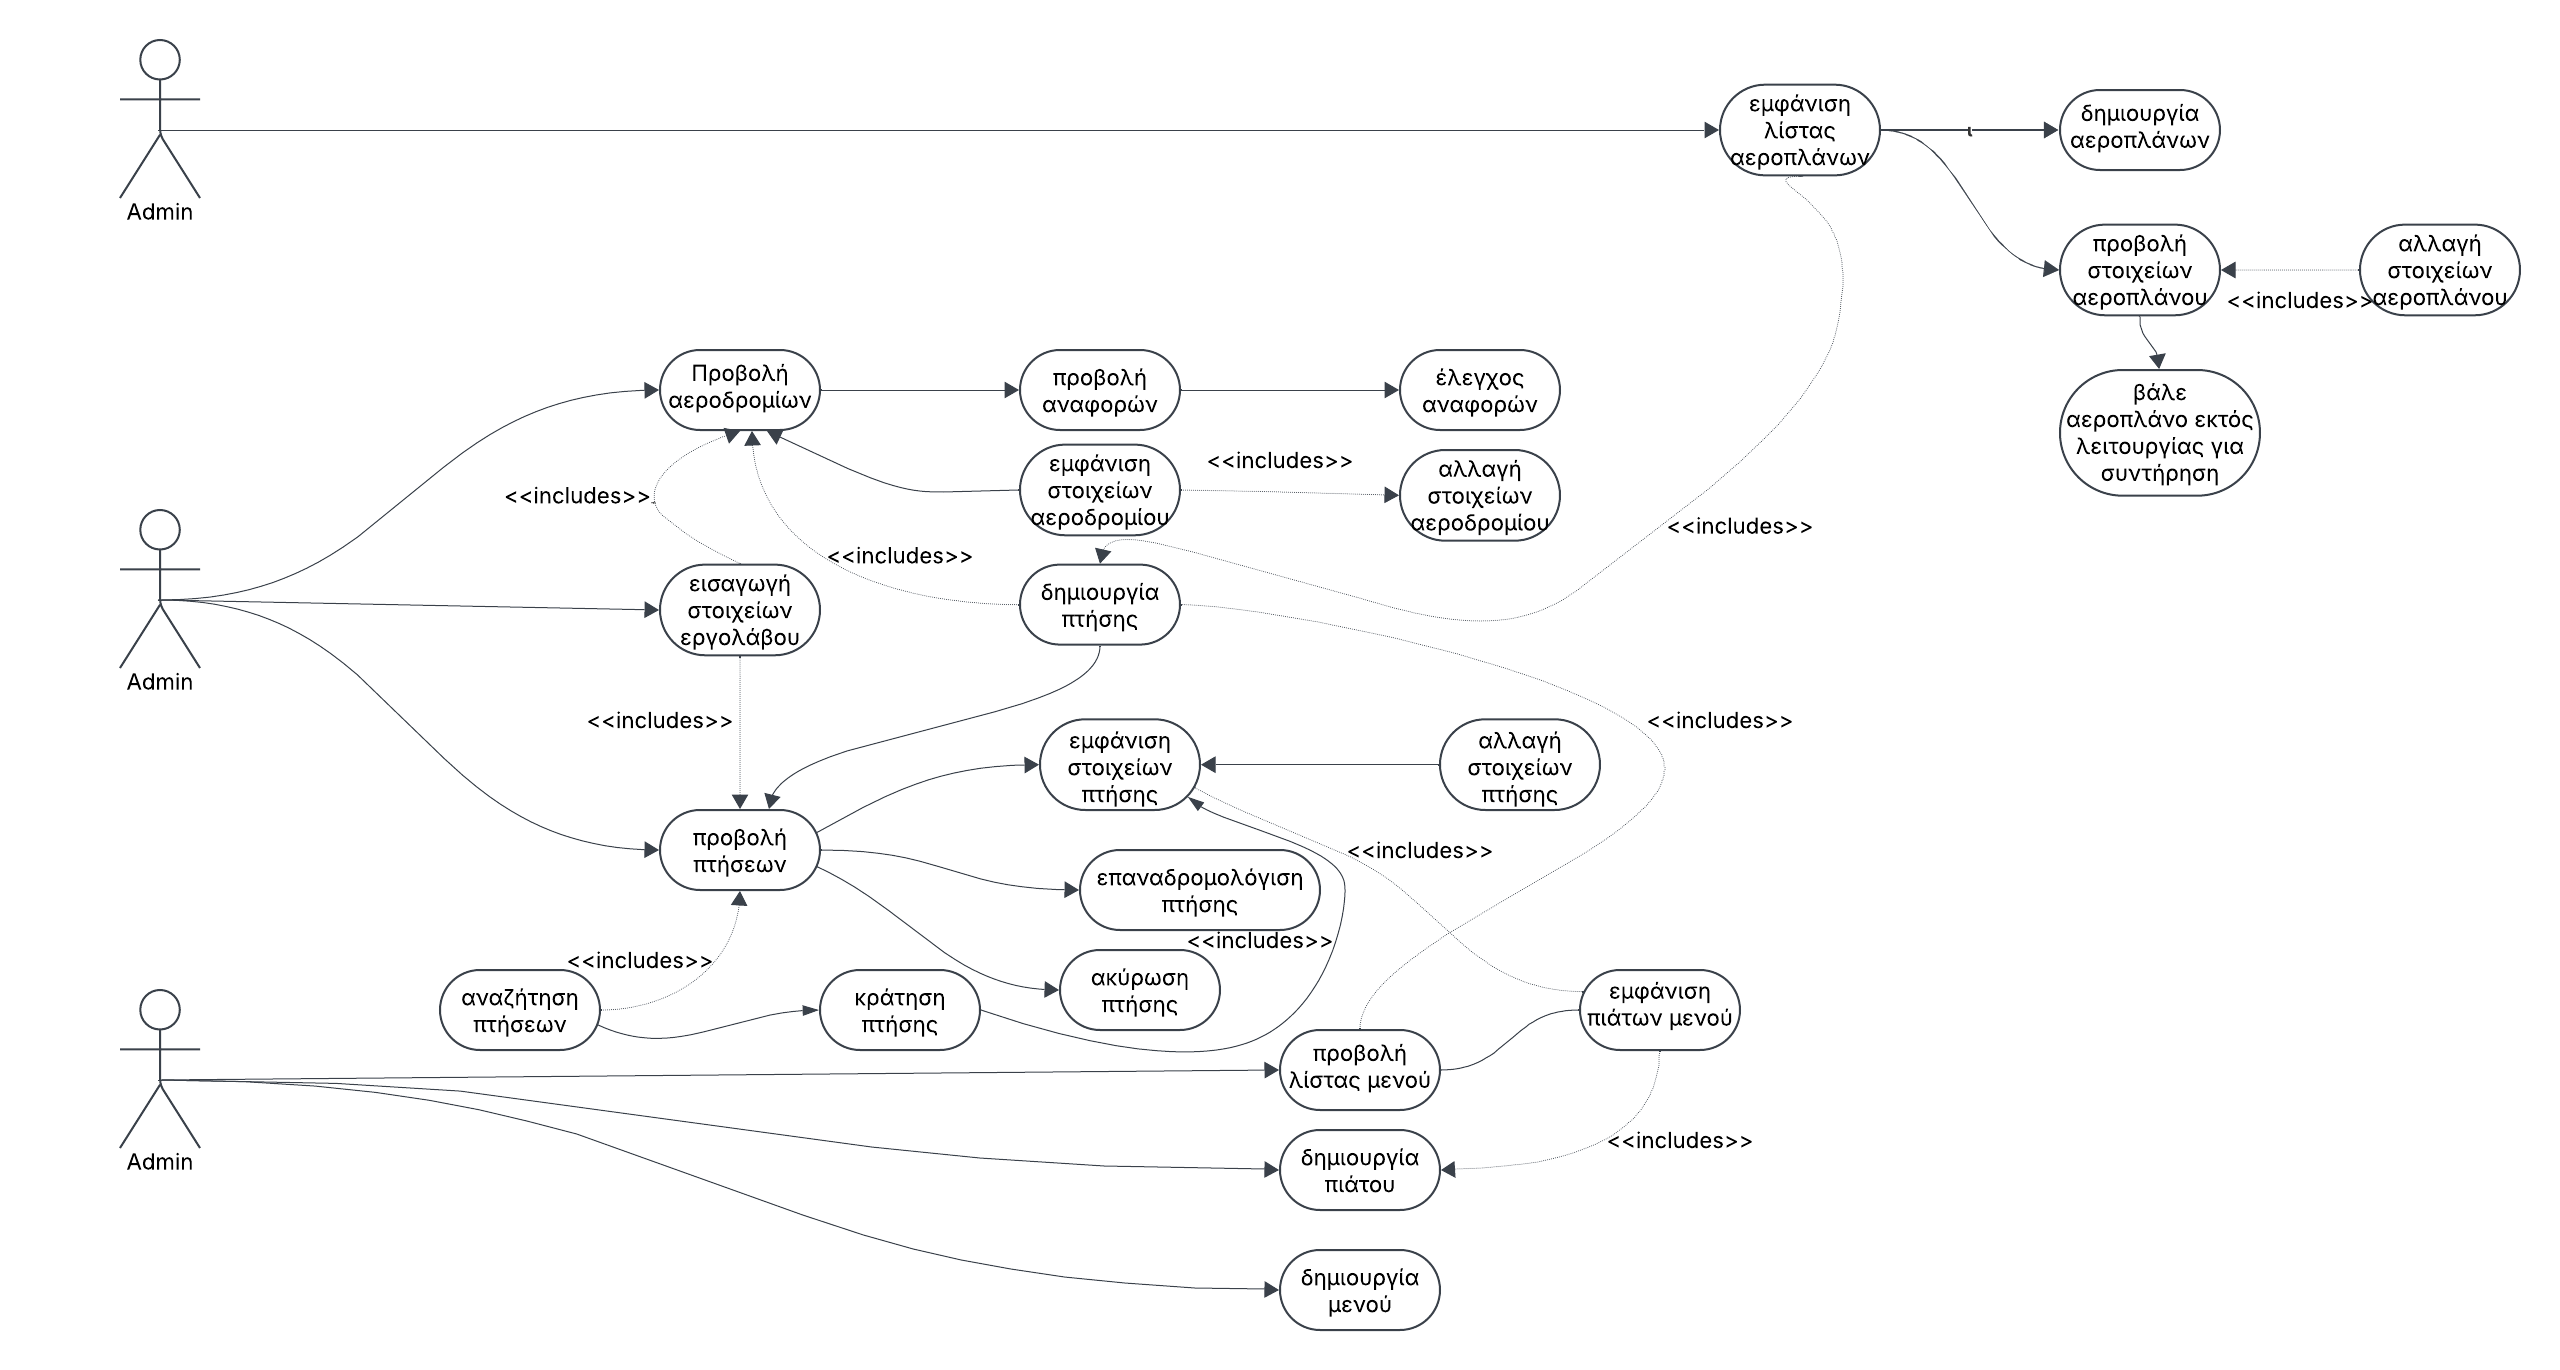
\includegraphics[width=\textwidth]{use-case-diagram.png}
\end{figure}

\section{Προβολή/Προσθήκη Πτήσεων}

\docChange{Σε αυτό το usecase έχω βάλει πολλά από τα βήματα στις ενναλλακτικές ροές στην βασική ροή}

% βασική ροή δημιουργίας πτήσης
\basicFlow
\begin{enumerate}
    \item Χρήστης επιλέγει "σχεδίαση πτήσης" \docChange{στην σελίδα προβολής πτήσης}
    \item \docChange{Σύστημα εμφανίζει την σελίδα Σχεδίαση Πτήσης}
    \item Χρήστης εισάγει τα στοιχεία της πτήσης που συμπεριλαμβάνει: τον αριθμό πτήσης, αεροδρόμιο αναχώρησης και άφιξης, χρόνους αναχώρησης και άφιξης 
    \item Το σύστημα εμφανίζει στην οθόνη όλα τα αεροπλάνα που μπορούν να εξυπηρετήσουν την πτήση στην ώρα που επέλεξε ο χρήστης. Δηλαδή να μπορούν να εξηπρετήσουν την πτήση χωρίς να συμπίπτει με τα άλλα δρομολόγια του και να μπορεί να πετάξει στα αεροδρόμια που επέλεξε ο χρήστης.
    \item\label{uc-step:plane-selected-for-flight} Χρήστης αν θέλει επιλέγει το αεροπλάνο που θα εξυπηρετήσει την πτήση
    \item \docChange{Αν έχει δωθεί αεροπλάνο στην πτήση} το σύστημα υπολογίζει ποιοι αεροσυνοδοί και πιλότοι είναι διαθέσιμοι για την πτήση αυτήν συμπεριλαμβάνοντας και τον χρόνο που χρειάζονται για να πάνε από την προηγούμενη πτήση στην επόμενη. Eπίσης ελέγχει να δει ότι έχουν την εξειδίκευση να δουλεύουν πάνω σε αυτό το αεροπλάνο.
    \item\label{uc-step:creation-of-flight-attendant} Ο χρήστης αν θέλει επιλέγει τους αεροσυνοδούς και τους πιλότους
    \item\label{uc-step:flight-submit-ready} χρήστης πατάει "ολοκλήρωση"
    \item To σύστημα βλέπει ότι έχουν συμπληρωθεί αρκετά στοιχεία για μια εγκεκριμένη πτήση και αποθηκεύει την πτήση με ετικέτα εγκεκριμένη
    \item Σύστημα αποθηκεύει αλλαγές και δείχνει την \docChange{σελίδα προβολή πτήσεων}
\end{enumerate}

% αποθήκευση draft πτήσης
\alternativeFlow
\flowbody{\ref{uc-step:flight-submit-ready}.a.}{
    \item Το σύστημα βλέπει ότι ο χρήστης δεν έχει επιλέξει όλες τις απαραίτητες πληροφορίες της πτήσης όπως επιλογή αεροσκάφος, πιλότων και αεροσυνοδών. Δεν επιτρέπει στον χρήστη να υποβάλει τις αλλαγές που έκανε.
}

% έχουν συμπληρωθεί αρκετά στοιχεία μόνο για ένα προσχέδιο πτήσης
\alternativeFlow
\begin{enumerate}[label=\ref{uc-step:flight-submit-ready}.b.\arabic*]
    \item To σύστημα βλέπει ότι έχουν συμπληρωθεί τα απαραίτητα στοιχεία για να δηλωθεί μια μη-εγκεκριμένη πτήση αλλά δεν έχουν συμπληρωθεί αρκετά στοιχεία για μια εγκεκριμένη πτήση και αποθηκεύει την πτήση με ετικέτα μη-εγκεκριμένη
\end{enumerate}


\section{Ακύρωση/Επαναδρομολόγηση Πτήσεων}

% ακύρωση πτήσης
\basicFlow
\flowbody{}{
    \item Χρήστης \docChange{επιλέγει} "προβολή πτήσεων"
    \item\label{uc-step:flight-list} Σύστημα εμφανίζει τις πτήσεις \docChange{στην οθόνη προβολή πτήσεων}
    \item Χρήστης φιλτράρει πτήσεις με το αν είναι προσχέδιο ή οριστικοποιημένη
    \item Σύστημα ενημερώνει την λίστα πτήσεων αν επέλεξε ο χρήστης φίλτρο
    \item\label{uc-step:flight-selected-from-list} Χρήστης επιλέγει πτήση
    \item \docChange{Σύστημα δείχνει την οθόνη προβολή στοιχείων πτήσης}
    \item Χρήστης \docChange{επιλέγει} αλλαγή στοιχείων
    \item Σύστημα εμφανίζει όλα τα στοιχεία της πτήσης \docChange{στην σελίδα αλλαγή στοιχείων πτήσης} και επιτρέπει στον χρήστη να αλλάξει ορισμένα στοιχείας της πτήσεις
    \item Χρήστης κάνει αλλαγές στα πεδία και επιλέγει αποθήκευση
    \item\label{uc-step:rescheduled-flight-changes-required} Σύστημα υπολογίζει αν οι αεροσυνοδοί, πιλότοι και αεροπλάνο θα είναι διαθέσιμοι να λειτουργήσουν την πτήση. Για κάθε οντότητα που δεν είναι διαθέσιμη θα αφαιρεθεί προσωσινά από την πτήση και \docChange{παρουσιάζει μήνυμα προειδοποίησης}
    \item Σύστημα αποθηκεύει τις αλλαγές και δεν αφήνει τον χρήστη να κάνει άλλες αλλαγές(εκτός αν ξανά επιλέξει αλλαγή στοιχείων)
}

% cancel flight
\alternativeFlow
\flowbody{\ref{uc-step:flight-selected-from-list}.a.}{
    \item \docChange{Στην οθόνη «Προβολή Πτήσης»} ο χρήστης επιλέγει «ακύρωσης πτήσης»
    \item Σύστημα υπολογίζει αν το αεροπλάνο της πτήσης θα πρέπει να επανατοποθετηθεί για να πραγματοποιηθεί η επόμενη πτήση αν αυτή η πτήση ακυρωθεί και το εμφανίζει ένα μήνυμα στην οθόνη.
    \item \docChange{Το σύστημα διαγράφει τους αεροσυνοδούς, πιλότους και το αεροπλάνο από την πτήση}
    \item Το σύστημα διαγράφει ολόκληρη την πτήση \docChange{και εμφανίζει μήνυμα επιτυχίας}
}


%menu use case
\section{Διαχείρηση menu}
% βασική ροή δημιουργίας menu
\bFlowIDReset
\basicFlow
\flowbody{}{
    \item\label{uc-step:menu creation} Ο χρήστης επιλέγει το κουμπί "εισαγωγή αντικειμένου menu"
    \item Το σύστημα δημιουργεί το νέο αντικείμενο
    \item Ο χρήστης εισάγει το όνομα, το κόστος και το βάρος του αντικειμένου
    \item\label{uc-step:cancel} Ο χρήστης επιλέγει το πλήκτρο καταχώρηση αντικειμένου
    \item Το σύστημα εισάγει το αντικείμενο στην λίστα των διαθέσιμων αντικειμένων μενού και επιστρέφει στην αρχική οθόνη
}

%εναλλακτική ροή ακύρωση εισαγωγής
\alternativeFlow
\flowbody{\ref{uc-step:cancel}.a.}{
    \item Ο χρήστης επιλέγει το πλήκτρο ακύρωση
    \item Το σύστημα διαγράφει το νέο αντικείμενο και επιστρέφει στην
    αρχική οθόνη
}

%εναλλακτική ροή δημιουργία μενού
\alternativeFlow
\flowbody{\ref{uc-step:menu creation}.a.}{
    \item Ο χρήστης επιλέγει το πλήκτρο δημιουργία μενού
    \item Το σύστημα εμφανίζει την οθόνη δημιουργία μενού και
    φορτώνει τα διαθέσιμα αντικείμενα μενού
    \item Ο χρήστης εισάγει τα στοιχεία του μενού, όνομα και μια μικρή περιγραφή για το ποιές πτήσεις αφορά \docChange{στην οθόνη δημιουργία μενου}
    \item Ο χρήστης επιλέγει το αντικείμενο που θέλει να προσθέσει
    στο μενού από τα διαθέσιμα αντικείμενα
    \item\label{uc-step:cancel item} Ο χρήστης επιλέγει το πλήκτρο εισαγωγή αντικειμένου
    \item Το σύστημα αποθηκεύει το αντικείμενο στο μενού. Τα
    βήματα 1.a.4-1.a.6 επαναλαμβάνονται όσο θέλει ο χρήστης
    \item\label{uc-step:cancel menu} Ο χρήστης επιλέγει το πλήκτρο καταχώρηση μενού
    \item \docChange{Το πρόγραμμα υπολογίζει την τιμή του μενού και το
    συνολικό του βάρος και εμφανίζει μια οθόνη στην οποία ο χρήστης μπορεί να αφαιρέσει αντικείμενα και να κάνει την τελική αποθήκευση του menu}
    \item το σύστημα αποθηκεύει στην λίστα με τα
    διαθέσιμα μενού. Το σύστημα επιστρέφει στην αρχική
    οθόνη
}

%εναλλακτική ροή ακύρωση εισαγωγής
\alternativeFlow
\flowbody{\ref{uc-step:cancel item}.}{
    \item Ο χρήστης επιλέγει το πλήκτρο ακύρωση
    \item  Το σύστημα ακυρώνει την εισαγωγή του στοιχείου και
επιστρέφει στο βήμα 1.a.4
}

%εναλλακτική ροή ακύρωση μενού
\alternativeFlow
\flowbody{\ref{uc-step:cancel menu}.}{
    \item Ο χρήστης επιλέγει το πλήκτρο ακύρωση μενού
    \item   Το σύστημα διαγράφει όλα τα στοιχεία του μενού και
    επιστρέφει στην αρχική οθόνη
}

\maketitle
\section{Διαχείριση Αναφορών πιλότων}

%Βασική ροή χειροκίνητος έλεγχος αναφορών
\bFlowIDReset
\basicFlow
\flowbody{}{
    \item Ο χρήστης επιλέγει το πλήκτρο ‘Διαχείριση αναφορών’
    \item Το σύστημα φορτώνει και εμφανίζει μια λίστα με όλα τα
    διαθέσιμα αεροπλάνα
    \item \label{back to main}Ο χρήστης επιλέγει ένα αεροπλάνο
    \item Το σύστημα εμφανίζει και φορτώνει όλες τις πτήσεις που έχουν
    εκτελεστεί με το αεροπλάνο
    \item\label{back to second screen} Ο χρήστης επιλέγει μία πτήση
    \item Το σύστημα φορτώνει και εμφανίζει την αναφορά των πιλότων
    μετά από την πτήση
    \item\label{back to third screen} Ο χρήστης επιλέγει το πλήκτρο ακύρωση πτήσεων
    \item Το πρόγραμμα ακυρώνει όλες τις προγραμματισμένες με αυτό
    το αεροπλάνο πτήσεις
}

%εναλλακτική ροή ακύρωση 1
\alternativeFlow
\flowbody{\ref{back to main}.a.}{
    \item Ο χρήστης επιλέγει το πλήκτρο ‘επιστροφή’
    \item Το σύστημα επιστρέφει στην αρχική οθόνη
}

%εναλλακτική ροή ακύρωση 2
\alternativeFlow
\flowbody{\ref{back to second screen}.a.}{
    \item Ο χρήστης επιλέγει το πλήκτρο επιστροφή
    \item Το σύστημα επιστρέφει στο βήμα 2 της βασικής ροής
}

%εναλλακτική ροή ακύρωση 3
\alternativeFlow
\flowbody{\ref{back to third screen}.a.}{
    \item  Ο χρήστης επιλέγει το πλήκτρο ‘επιστροφή
    \item Το σύστημα επιστρέφει στο βήμα 4 της βασικής ροής
}

\section{Διαχείριση αεροδρομίων }
%βασική ροή πίνακας αεροδρομίων 
\bFlowIDReset
\basicFlow
\flowbody{}{
    \item Χρήστης επιλέγει τη διαχείριση αεροδρομίων από το σύστημα.
    \item Το σύστημα εμφανίζει λίστα με όλα τα αεροδρόμια που χρησιμοποιεί η αεροπορική εταιρεία.
    \item \label{back to airport list} Χρήστης επιλέγει ένα αεροδρόμιο για προβολή ή επεξεργασία.
    \item Το σύστημα εμφανίζει λεπτομέρειες για το επιλεγμένο αεροδρόμιο, όπως τοποθεσία, χωρητικότητα, ωράριο λειτουργίας, μέγιστος αριθμός πτήσεων, αριθμός διαδρόμων  και μέγιστο μήκος διαδρόμου.
    \item \label{back to airport} Χρήστης μπορεί να τροποποιήσει στοιχεία του αεροδρομίου, όπως ωράριο λειτουργίας ή μέγιστο αριθμό πτήσεων.
    \item Χρήστης επιβεβαιώνει τις αλλαγές.
    \item Το σύστημα αποθηκεύει τις αλλαγές και ενημερώνει τα σχετικά δεδομένα πτήσεων αν χρειάζεται.
}

%εναλλακτική ροή  1
\alternativeFlow
\flowbody{\ref{back to airport list}.a.}{
    \item Ο χρήστης επιλέγει το πλήκτρο ‘επιστροφή’
    \item Το σύστημα επιστρέφει στην αρχική οθόνη
}

%εναλλακτική ροή  2
\alternativeFlow
\flowbody{\ref{back to airport list}.b.}{

    \item Το Χρήστης επιλέγει να προσθέσει νέο αεροδρόμιο.
    \item Το Το σύστημα εμφανίζει φόρμα καταχώρησης νέου αεροδρομίου.
    \item Το Χρήστης συμπληρώνει τα στοιχεία του αεροδρομίου όπως όνομα, μέγιστη χωρητικότητα, αριθμοί διαδρόμων κτλ.
    \item Το Χρήστης πατάει επιβεβαίωση.
    \item Το Το σύστημα καταχωρεί το νέο αεροδρόμιο στη βάση δεδομένων και ενημερώνει τις διαθέσιμες επιλογές δρομολογίων.
}

%εναλλακτική ροή 3
\alternativeFlow
\flowbody{\ref{back to airport}.a.}{

    \item Χρήστης επιλέγει να διαγράψει ένα αεροδρόμιο.
    \item Το σύστημα ελέγχει αν το αεροδρόμιο είναι ενεργό.
    \item Το σύστημα εμφανίζει προειδοποιητικό μήνυμα και δεν επιτρέπει τη διαγραφή σε περίπτωση που είναι ενεργό.
    \item Το σύστημα ζητά επιβεβαίωση από τον χρήστη.
    \item Χρήστης επιβεβαιώνει τη διαγραφή.
    \item Το σύστημα αφαιρεί το αεροδρόμιο από τη βάση δεδομένων.
}


%εναλλακτική ροή  4
\alternativeFlow
\flowbody{\ref{back to airport}.b.}{

    \item Ο χρήστης μπορεί να επισημάνει το αεροδρόμιο ως ανενεργό.
    \item Το σύστημα ενημερώνει αυτόματα όλα τα δρομολόγια που το περιλαμβάνουν και τα χαρακτηρίζει ως μη πραγματοποιήσιμα.
    \item Το σύστημα ειδοποιεί τον διαχειριστή πτήσεων για να αναθέσει εναλλακτικά αεροδρόμια όπου χρειάζεται.
    \item Επιστροφή στη βασική ροή.
}

%εναλλακτική ροή  5
\alternativeFlow
\flowbody{\ref{back to airport}.c.}{
    \item Ο χρήστης επιλέγει το πλήκτρο επιστροφή
    \item Το σύστημα επιστρέφει στο βήμα 2 της βασικής ροής
}
\docChange{
%εναλλακτική ροή  6
\alternativeFlow
\flowbody{\ref{back to airport}.d.}{
    \item Ο χρήστης εισάγει μη έγκυρα στοιχεία
    \item Το σύστημα εμφανίζει μια προειδοποιητικη οθόνη και δεν επιτρέπει την υποβολή στον χρήστη
}
}
\section{Διαχείριση υπαλλήλων }

%βασική ροή πίνακας υπαλλήλων  
\bFlowIDReset
\basicFlow
\flowbody{}{
    \item Ο χρήστης επιλέγει τη διαχείριση εργαζομένων από το σύστημα.
    \item Το σύστημα εμφανίζει λίστα με όλους τους εργαζομένους της εταιρείας (π.χ., πιλότοι, αεροσυνοδοί, μηχανικοί, διαχειριστές εδάφους).
    \item \label{back to employee list} Ο χρήστης επιλέγει έναν εργαζόμενο για προβολή ή επεξεργασία.
    \item Το σύστημα εμφανίζει λεπτομέρειες του επιλεγμένου εργαζομένου όπως  ID, ηλικία, θέσης εργασίας, ώρες εργασίας κλπ..
    \item \label{back to employee} Ο χρήστης επεξεργάζεται τις πληροφορίες, αν χρειάζεται.
    \item Ο χρήστης επιβεβαιώνει τις αλλαγές.
    \item Το σύστημα αποθηκεύει τις αλλαγές και ενημερώνει τυχόν σχετικές πτήσεις, δρομολόγια ή προγράμματα εργασίας.
}

%βασική ροή πίνακας φίλτρο  
\bFlowIDReset
\basicFlow
\flowbody{}{
    \item Ο χρήστης επιλέγει να προβάλλει διαθέσιμους υπαλλήλους .
    \item Το σύστημα εμφανίζει φίλτρα αναζήτησης, όπως όνομα , ηλικία, δουλειά.
    \item Ο χρήστης επιλέγει τις επιθυμητές παραμέτρους και εκτελεί την αναζήτηση.
    \item Το σύστημα εμφανίζει τη λίστα των διαθέσιμων υπαλλήλους  που ταιριάζουν στα κριτήρια.
    \item Ο χρήστης μπορεί να επιλέξει έναν υπάλληλο για προβολή λεπτομερειών.
    \item Επιστροφή στο μενού διαχείρισης αεροσκαφών.
}

%εναλλακτική ροή 1
\alternativeFlow
\flowbody{\ref{back to employee list}.a.}{
    \item Ο χρήστης επιλέγει το πλήκτρο ‘επιστροφή’
    \item Το σύστημα επιστρέφει στην αρχική οθόνη
}

%εναλλακτική ροή 2
\alternativeFlow
\flowbody{\ref{back to employee list}.b.}{
    \item Ο χρήστης επιλέγει να προσθέσει έναν νέο εργαζομένου.
    \item Το σύστημα εμφανίζει φόρμα εισαγωγής νέου εργαζομένου.
    \item Ο χρήστης συμπληρώνει τα στοιχεία του εργαζομένου
    \item Ο χρήστης επιβεβαιώνει την εισαγωγή.
    \item Το σύστημα καταχωρεί τον νέο εργαζόμενο στη βάση δεδομένων και τον καθιστά διαθέσιμο για μελλοντικές αναθέσεις εργασιών.
}

%εναλλακτική ροή 3
\alternativeFlow
\flowbody{\ref{back to employee}.a.}{
    \item Ο χρήστης επιλέγει να διαγράψει έναν εργαζόμενο.
    \item Το σύστημα ελέγχει αν ο εργαζόμενος είναι ενεργός .
    \item Το σύστημα εμφανίζει προειδοποιητικό μήνυμα και δεν επιτρέπει τη διαγραφή αν ο εργαζόμενος είναι ενεργός.
    \item Αν δεν είναι ενεργός , το σύστημα ζητά επιβεβαίωση από τον χρήστη.
    \item Ο χρήστης επιβεβαιώνει τη διαγραφή.
    \item Το σύστημα αφαιρεί τον εργαζόμενο από τη βάση δεδομένων.
}

%εναλλακτική ροή 4
\alternativeFlow
\flowbody{\ref{back to employee}.b.}{
    \item Ο χρήστης επιλέγει να αλλάξει τους περιορισμούς ενός τύπου εργαζομένου όπως μέγιστες ώρες εργασίας ανά εβδομάδα, απαιτούμενες άδειες.
    \item Το σύστημα ελέγχει αν υπάρχουν εργαζόμενοι που επηρεάζονται από την αλλαγή.
    \item Το σύστημα εμφανίζει ειδοποίηση με τις πιθανές επιπτώσεις όπως ανάγκη για αλλαγές σε βάρδιες ή πτήσεις.
    \item Ο χρήστης επιβεβαιώνει την αλλαγή.
    \item Το σύστημα ενημερώνει τα προγράμματα εργασίας των εργαζομένων που επηρεάζονται.
    \item Επιστροφή στη βασική ροή.
}

%εναλλακτική ροή 5
\alternativeFlow
\flowbody{\ref{back to employee}.c.}{
    \item Ο χρήστης επιλέγει να επισημάνει έναν τύπο εργαζομένου ως μη διαθέσιμο προσωρινά.
    \item Το σύστημα ενημερώνει αυτόματα τα προγράμματα εργασίας και τις πτήσεις, αποδεσμεύοντας προσωρινά τους εργαζομένους αυτού του τύπου.
    \item Αν απαιτείται αντικατάσταση, το σύστημα ειδοποιεί τον διαχειριστή για την ανάγκη εύρεσης εναλλακτικού προσωπικού.
    \item Επιστροφή στη βασική ροή.

}

%εναλλακτική ροή 6
\alternativeFlow
\flowbody{\ref{back to  employee}.d.}{
    \item Ο χρήστης επιλέγει το πλήκτρο επιστροφή
    \item Το σύστημα επιστρέφει στο βήμα 2 της βασικής ροής
}
\docChange{
%εναλλακτική ροή  7
\alternativeFlow
\flowbody{\ref{back to employee}.e.}{
    \item Ο χρήστης εισάγει μη έγκυρα στοιχεία
    \item Το σύστημα εμφανίζει μια προειδοποιητικη οθόνη και δεν επιτρέπει την υποβολή στον χρήστη
}
}
\section{Διαχείριση αεροπλάνων}

%βασική ροή πίνακας αεροπλάνων 
\bFlowIDReset
\basicFlow
\flowbody{}{
    \item Ο χρήστης επιλέγει τη διαχείριση τύπων αεροσκαφών από το σύστημα.
    \item Το σύστημα εμφανίζει λίστα με όλους τους τύπους αεροσκαφών που χρησιμοποιεί η εταιρεία.
    \item \label{back to airplane list} Ο χρήστης επιλέγει έναν τύπο αεροσκάφους για προβολή ή επεξεργασία.
    \item Το σύστημα εμφανίζει λεπτομέρειες για το επιλεγμένο αεροσκάφος, όπως τύπος αεροσκάφους, χωρητικότητα επιβατών, μέγιστο φορτίο κλπ..
    \item \label{back to airplane} Ο χρήστης επεξεργάζεται τις πληροφορίες αν χρειάζεται.
    \item Ο χρήστης επιβεβαιώνει τις αλλαγές.
    \item Το σύστημα αποθηκεύει τις αλλαγές και ενημερώνει τα σχετικά δεδομένα πτήσεων αν χρειάζεται.
}

%βασική ροή πίνακας φίλτρο  
\bFlowIDReset
\basicFlow
\flowbody{}{ 
    \item Ο χρήστης επιλέγει να προβάλλει διαθέσιμα αεροσκάφη.
    \item Το σύστημα εμφανίζει φίλτρα αναζήτησης, όπως χωρητικότητα επιβατών, εμβέλεια πτήσης, τύπος αεροσκάφους
    \item Ο χρήστης επιλέγει τις επιθυμητές παραμέτρους και εκτελεί την αναζήτηση.
    \item Το σύστημα εμφανίζει τη λίστα των διαθέσιμων αεροσκαφών που ταιριάζουν στα κριτήρια.
    \item Ο χρήστης μπορεί να επιλέξει ένα αεροσκάφος για προβολή λεπτομερειών.
    \item Επιστροφή στο μενού διαχείρισης αεροσκαφών.
}

%εναλλακτική ροή 1
\alternativeFlow
\flowbody{\ref{back to airplane list}.a.}{
    \item Ο χρήστης επιλέγει το πλήκτρο ‘επιστροφή’
    \item Το σύστημα επιστρέφει στην αρχική οθόνη
}


%εναλλακτική ροή 2
\alternativeFlow
\flowbody{\ref{back to airplane list}.b.}{
    \item Ο χρήστης επιλέγει να προσθέσει έναν νέο τύπο αεροσκάφους.
    \item Το σύστημα εμφανίζει φόρμα εισαγωγής νέου τύπου αεροσκάφους.
    \item Ο χρήστης συμπληρώνει τα στοιχεία του αεροσκάφους (τύπος, χωρητικότητα, μέγιστο φορτίο, εμβέλεια κτλ.).
    \item Ο χρήστης επιβεβαιώνει την εισαγωγή.
    \item Το σύστημα καταχωρεί το νέο αεροσκάφος στη βάση δεδομένων και το καθιστά διαθέσιμο για μελλοντικά δρομολόγια.
}

%εναλλακτική ροή 3
\alternativeFlow
\flowbody{\ref{back to airplane}.a.}{
   \item Ο χρήστης επιλέγει να διαγράψει έναν τύπο αεροσκάφους.
   \item Το σύστημα ελέγχει αν το αεροσκάφος είναι ενεργό.
   \item Το σύστημα εμφανίζει προειδοποιητικό μήνυμα και δεν επιτρέπει τη διαγραφή αν είναι ενεργό.
   \item Το σύστημα ζητά επιβεβαίωση από τον χρήστη.
   \item Ο χρήστης επιβεβαιώνει τη διαγραφή.
   \item Το σύστημα αφαιρεί το αεροσκάφος από τη βάση δεδομένων.
}


%εναλλακτική ροή 4
\alternativeFlow
\flowbody{\ref{back to airplane}.b.}{
   \item Ο χρήστης μπορεί να επισημάνει ένα αεροσκάφος ως ανενεργό.
   \item Το σύστημα ενημερώνει αυτόματα όλα τα δρομολόγια που το περιλαμβάνουν και τα χαρακτηρίζει ως μη πραγματοποιήσιμα.
   \item Το σύστημα ειδοποιεί τον διαχειριστή πτήσεων να αναθέσει εναλλακτικά αεροσκάφη όπου χρειάζεται.
   \item Επιστροφή στη βασική ροή.
}

%εναλλακτική ροή 5
\alternativeFlow
\flowbody{\ref{back to  airplane}.c.}{
    \item Ο χρήστης επιλέγει το πλήκτρο επιστροφή
    \item Το σύστημα επιστρέφει στο βήμα 2 της βασικής ροής
}

\docChange{
%εναλλακτική ροή  6
\alternativeFlow
\flowbody{\ref{back to airplane}.d.}{
    \item Ο χρήστης εισάγει μη έγκυρα στοιχεία
    \item Το σύστημα εμφανίζει μια προειδοποιητικη οθόνη και δεν επιτρέπει την υποβολή στον χρήστη
}
}
%Βασική ροή Ανάθεση Εργολάβων στο Αεροδρόμιο 

\section{Ανάθεση εργασίας σε εργολάβους}
\bFlowIDReset
\basicFlow
\flowbody{}{
    \item Ο διαχειριστής επιλέγει το πλήκτρο "ανάθεση εργασίας σε εργολάβο"
    \item Το σύστημα φορτώνει την σελίδα εισαγωγής πληροφοριών για την εργασία
    \item Ο διαχειριστής εισάγει τα στοιχεία της εργασίας που θέλει να γίνει
    \item\label{cancel page 1} Ο χρήστης επιλέγει το πλήκτρο "continue" και το σύστημα φορτώνει τους διαθέσιμους εργολάβους για εκείνο το αεροδρόμιο με πληροφορίες για την δουλειά και την χρέωσή τους.
    \item\label{cancel page 2} Ο χρήστης επιλέγει εργολάβο
    \item Το σύστημα φορτώνει μια σελίδα με όλες τις πληροφορίες για την εργασία και τις πληροφορίες του εργολάβου που έχει επιλεγεί
    \item \label{cancel page 3} Ο διαχειριστής εγκρίνει την συνεργασία 
    \item Το σύστημα καταχωρεί την συνεργασία

}

% Επιστροφή οθόνη 1
\alternativeFlow
\flowbody{\ref{cancel page 1}.a.}{
    \item Ο χρήστης επιλέγει το πλήκτρο επιστροφή
    \item Το σύστημα επιστρέφει στην αρχική οθόνη
}

%Επιστροφή οθόνη 2
\alternativeFlow
\flowbody{\ref{cancel page 2}.a.}{
    \item Ο χρήστης επιλέγει το πλήκτρο επιστροφή
    \item Το σύστημα επιστρέφει στην προηγούμενη οθόνη
}

%Εμφάνιση ενεργών συνεργασιών
\alternativeFlow
\flowbody{\ref{cancel page 2}.b.}{
    \item Ο χρήστης επιλέγει το πλήκτρο εμφάνιση contructs
    \item Το σύστημα φορτώνει την σελίδα με τα cintructs που τρέχουν
    \item Ο χρήστης επιλέγει μια συνεργασία και επιλέγει την ολοκλήρωσή της
    \item Το σύστημα φορτώνει μια οθόνη ολοκλήρωσης και ο χρήστης επιλέγει την πληρωμή του contruct
}

%Επιστροφή οθόνη 3
\alternativeFlow
\flowbody{\ref{cancel page 3}.a.}{
    \item Ο χρήστης επιλέγει το πλήκτρο επιστροφή
    \item Το σύστημα επιστρέφει στην προηγούμενη οθόνη 
}
% Αναζήτηση Πτήσης
\section{Αγορά Εισητηρίου}
\bFlowIDReset
\basicFlow
\flowbody{}{
    \item Ο χρήστης επιλέγει την ενότητα "Αναζήτηση Πτήσης" \docChange{στην κύρια οθόνη}
    \item\label{uc-step:search-plane-with-filter} \docChange{Στην οθόνη αναζήτησης πτήσης ο χρήστης επιλέγει φίλτρα για την αναζήτηση πτήσεων}
    \item Το σύστημα εμφανίζει \docChange{την οθόνη αναζήτησης πτήσης} εμαφανίζει διαθέσιμες πτήσεις με ώρα, τιμή, αριθμό πτήσης και συνοπτική περιγραφή.
    \item\label{uc-step:user buys} Ο χρήστης επιλέγει πτήση 
    \item Το σύστημα εμφανίζει περίληψη πτήσης και πεδία εισαγωγής στοιχείων επιβατών.
    \item\label{uc-step:fill-passenger-data} Ο χρήστης συμπληρώνει για κάθε επιβάτη: Όνομα, Επώνυμο, Email, Ημερομηνία Γέννησης, Αρ. Διαβατηρίου.
    \item Το σύστημα \docChange{κάνει έλεγχο για τα στοιχεία του επιβάτη}, υπολογίζει και εμφανίζει την τελική τιμή κράτησης και \docChange{δείχνει την οθόνη επιτυχής κράτηση}.
    \item Ο χρήστης πατάει «Οριστικοποίηση Κράτησης».
    \item Το σύστημα αποθηκεύει την κράτηση και εμφανίζει μήνυμα επιτυχίας και τα στοιχεία της κράτησης
    \item Σημείωση εμφανίζεται στην οθόνη: «Η πληρωμή πραγματοποιείται από τον gate agent πριν την επιβίβαση.»
}

\alternativeFlow
\flowbody{\ref{uc-step:user buys}.a.}{
    \item Ο χρήστης προσπαθεί να επιλέξει πτήση που μόλις έγινε sold out.
    \item Το σύστημα εμφανίζει μήνυμα «Η πτήση δεν είναι πλέον διαθέσιμη».
    \item Ο χρήστης επιλέγει άλλη πτήση και η ροή συνεχίζεται από το βήμα 3.
}

\alternativeFlow
\flowbody{\ref{uc-step:search-plane-with-filter}}{
    \item \docChange{αν δεν υπάρχουν πτήσεις με αυτό το φίλτρο το σύστημα εμφανίζει σφάλμα}
}

% Συντήρηση Αεροσκαφών
\section{Συντήρηση αεροσκαφών}
\bFlowIDReset
\basicFlow
\flowbody{}{
    \item Επιλέγει την ενότητα "Συντήρηση Αεροσκαφών"
    \item\label{uc-step:display plane list} Το σύστημα εμφανίζει λίστα με τα μη διαθέσιμα αεροσκάφη.
    \item Ο διαχειριστής επιλέγει αεροσκάφος.
    \item\label{uc-step:show future flights} Εμφανίζονται οι μελλοντικές πτήσεις του και η αναφορά με την οποια το αεροσκάφος μπήκε ανενεργό.
    \item\label{uc-step:maintenance date} Ο διαχειριστής ορίζει ημερομηνίες συντήρησης.
    \item Αν δεν υπάρχουν συγκρούσεις,\docChange{το σύστημα αποθηκεύει την ημερομηνία και εμφανίζει στον χρήστη οθόνη επιβεβαίωσης
}
}

\alternativeFlow
\flowbody{\ref{uc-step:display plane list}.a.}{
    \item Δεν υπάρχουν διαθέσιμα αεροσκάφη.
    \item Εμφανίζεται μήνυμα και η διαδικασία ακυρώνεται.
}

\alternativeFlow
\flowbody{\ref{uc-step:show future flights}.a.}{
    \item Το επιλεγμένο αεροσκάφος δεν έχει προγραμματισμένες πτήσεις.
    \item \docChange{Εμφανίζεται μήνυμα και η διαδικασία ακυρώνεται.}
}

\alternativeFlow
\flowbody{\ref{uc-step:maintenance date}.a.}{
    \item Η ημερομηνία έναρξης συντήρησης είναι μετά τη λήξη.
    \item Το σύστημα εμφανίζει προειδοποίηση και ζητά διόρθωση.
}

\end{document}
